\documentclass[1p]{elsarticle_modified}
%\bibliographystyle{elsarticle-num}

%\usepackage[colorlinks]{hyperref}
%\usepackage{abbrmath_seonhwa} %\Abb, \Ascr, \Acal ,\Abf, \Afrak
\usepackage{amsfonts}
\usepackage{amssymb}
\usepackage{amsmath}
\usepackage{amsthm}
\usepackage{scalefnt}
\usepackage{amsbsy}
\usepackage{kotex}
\usepackage{caption}
\usepackage{subfig}
\usepackage{color}
\usepackage{graphicx}
\usepackage{xcolor} %% white, black, red, green, blue, cyan, magenta, yellow
\usepackage{float}
\usepackage{setspace}
\usepackage{hyperref}

\usepackage{tikz}
\usetikzlibrary{arrows}

\usepackage{multirow}
\usepackage{array} % fixed length table
\usepackage{hhline}

%%%%%%%%%%%%%%%%%%%%%
\makeatletter
\renewcommand*\env@matrix[1][\arraystretch]{%
	\edef\arraystretch{#1}%
	\hskip -\arraycolsep
	\let\@ifnextchar\new@ifnextchar
	\array{*\c@MaxMatrixCols c}}
\makeatother %https://tex.stackexchange.com/questions/14071/how-can-i-increase-the-line-spacing-in-a-matrix
%%%%%%%%%%%%%%%

\usepackage[normalem]{ulem}

\newcommand{\msout}[1]{\ifmmode\text{\sout{\ensuremath{#1}}}\else\sout{#1}\fi}
%SOURCE: \msout is \stkout macro in https://tex.stackexchange.com/questions/20609/strikeout-in-math-mode

\newcommand{\cancel}[1]{
	\ifmmode
	{\color{red}\msout{#1}}
	\else
	{\color{red}\sout{#1}}
	\fi
}

\newcommand{\add}[1]{
	{\color{blue}\uwave{#1}}
}

\newcommand{\replace}[2]{
	\ifmmode
	{\color{red}\msout{#1}}{\color{blue}\uwave{#2}}
	\else
	{\color{red}\sout{#1}}{\color{blue}\uwave{#2}}
	\fi
}

\newcommand{\Sol}{\mathcal{S}} %segment
\newcommand{\D}{D} %diagram
\newcommand{\A}{\mathcal{A}} %arc


%%%%%%%%%%%%%%%%%%%%%%%%%%%%%5 test

\def\sl{\operatorname{\textup{SL}}(2,\Cbb)}
\def\psl{\operatorname{\textup{PSL}}(2,\Cbb)}
\def\quan{\mkern 1mu \triangleright \mkern 1mu}

\theoremstyle{definition}
\newtheorem{thm}{Theorem}[section]
\newtheorem{prop}[thm]{Proposition}
\newtheorem{lem}[thm]{Lemma}
\newtheorem{ques}[thm]{Question}
\newtheorem{cor}[thm]{Corollary}
\newtheorem{defn}[thm]{Definition}
\newtheorem{exam}[thm]{Example}
\newtheorem{rmk}[thm]{Remark}
\newtheorem{alg}[thm]{Algorithm}

\newcommand{\I}{\sqrt{-1}}
\begin{document}

%\begin{frontmatter}
%
%\title{Boundary parabolic representations of knots up to 8 crossings}
%
%%% Group authors per affiliation:
%\author{Yunhi Cho} 
%\address{Department of Mathematics, University of Seoul, Seoul, Korea}
%\ead{yhcho@uos.ac.kr}
%
%
%\author{Seonhwa Kim} %\fnref{s_kim}}
%\address{Center for Geometry and Physics, Institute for Basic Science, Pohang, 37673, Korea}
%\ead{ryeona17@ibs.re.kr}
%
%\author{Hyuk Kim}
%\address{Department of Mathematical Sciences, Seoul National University, Seoul 08826, Korea}
%\ead{hyukkim@snu.ac.kr}
%
%\author{Seokbeom Yoon}
%\address{Department of Mathematical Sciences, Seoul National University, Seoul, 08826,  Korea}
%\ead{sbyoon15@snu.ac.kr}
%
%\begin{abstract}
%We find all boundary parabolic representation of knots up to 8 crossings.
%
%\end{abstract}
%\begin{keyword}
%    \MSC[2010] 57M25 
%\end{keyword}
%
%\end{frontmatter}

%\linenumbers
%\tableofcontents
%
\newcommand\colored[1]{\textcolor{white}{\rule[-0.35ex]{0.8em}{1.4ex}}\kern-0.8em\color{red} #1}%
%\newcommand\colored[1]{\textcolor{white}{ #1}\kern-2.17ex	\textcolor{white}{ #1}\kern-1.81ex	\textcolor{white}{ #1}\kern-2.15ex\color{red}#1	}

{\Large $\underline{10_{88}~(K10a_{11})}$}

\setlength{\tabcolsep}{10pt}
\renewcommand{\arraystretch}{1.6}
\vspace{1cm}\begin{tabular}{m{100pt}>{\centering\arraybackslash}m{274pt}}
\multirow{5}{120pt}{
	\centering
	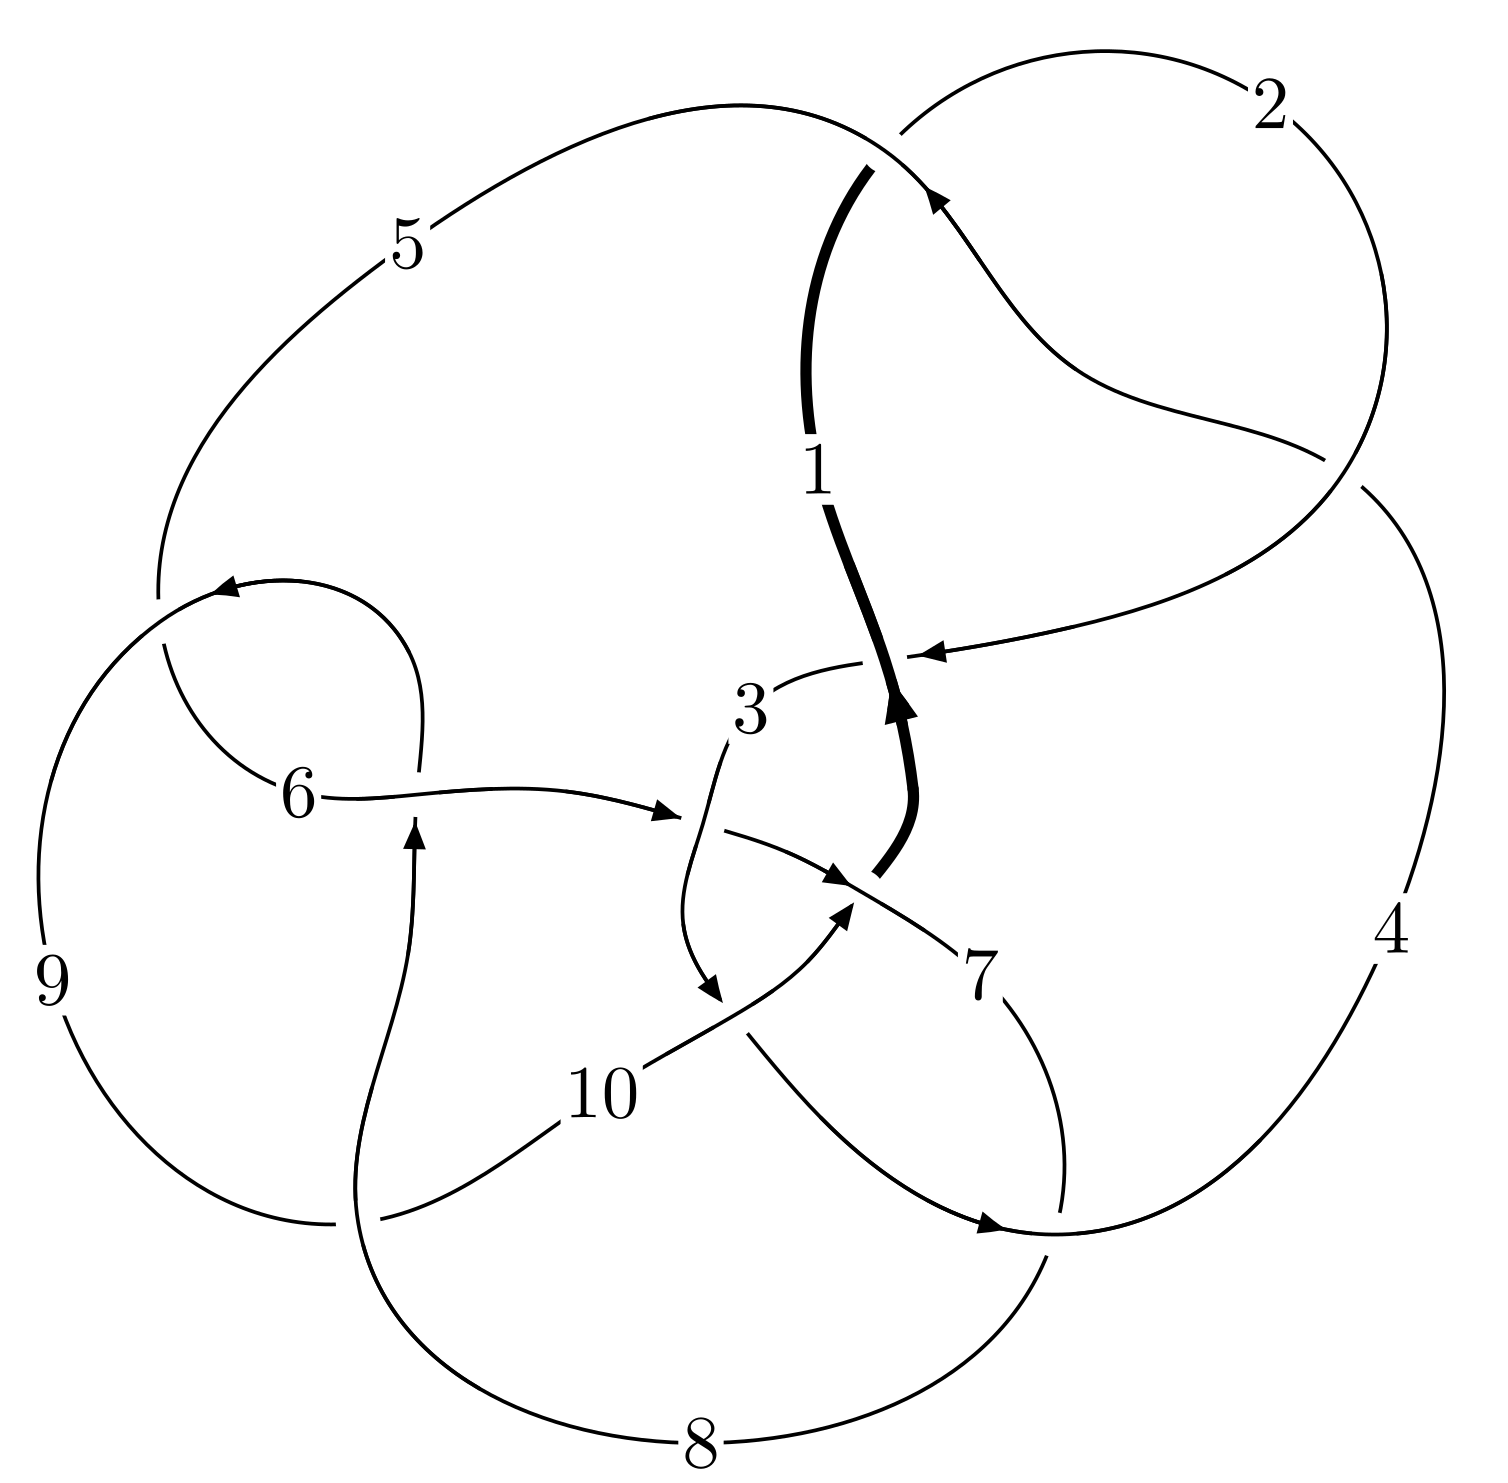
\includegraphics[width=112pt]{../../../GIT/diagram.site/Diagrams/png/172_10_88.png}\\
\ \ \ A knot diagram\footnotemark}&
\allowdisplaybreaks
\textbf{Linearized knot diagam} \\
\cline{2-2}
 &
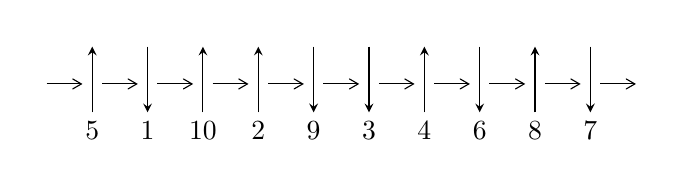
\begin{tikzpicture}[x=20pt, y=17pt]
	% nodes
	\node (C0) at (0, 0) {};
	\node (C1) at (1, 0) {};
	\node (C1U) at (1, +1) {};
	\node (C1D) at (1, -1) {5};

	\node (C2) at (2, 0) {};
	\node (C2U) at (2, +1) {};
	\node (C2D) at (2, -1) {1};

	\node (C3) at (3, 0) {};
	\node (C3U) at (3, +1) {};
	\node (C3D) at (3, -1) {10};

	\node (C4) at (4, 0) {};
	\node (C4U) at (4, +1) {};
	\node (C4D) at (4, -1) {2};

	\node (C5) at (5, 0) {};
	\node (C5U) at (5, +1) {};
	\node (C5D) at (5, -1) {9};

	\node (C6) at (6, 0) {};
	\node (C6U) at (6, +1) {};
	\node (C6D) at (6, -1) {3};

	\node (C7) at (7, 0) {};
	\node (C7U) at (7, +1) {};
	\node (C7D) at (7, -1) {4};

	\node (C8) at (8, 0) {};
	\node (C8U) at (8, +1) {};
	\node (C8D) at (8, -1) {6};

	\node (C9) at (9, 0) {};
	\node (C9U) at (9, +1) {};
	\node (C9D) at (9, -1) {8};

	\node (C10) at (10, 0) {};
	\node (C10U) at (10, +1) {};
	\node (C10D) at (10, -1) {7};
	\node (C11) at (11, 0) {};

	% arrows
	\draw[->,>={angle 60}]
	(C0) edge (C1) (C1) edge (C2) (C2) edge (C3) (C3) edge (C4) (C4) edge (C5) (C5) edge (C6) (C6) edge (C7) (C7) edge (C8) (C8) edge (C9) (C9) edge (C10) (C10) edge (C11) ;	\draw[->,>=stealth]
	(C1D) edge (C1U) (C2U) edge (C2D) (C3D) edge (C3U) (C4D) edge (C4U) (C5U) edge (C5D) (C6U) edge (C6D) (C7D) edge (C7U) (C8U) edge (C8D) (C9D) edge (C9U) (C10U) edge (C10D) ;
	\end{tikzpicture} \\
\hhline{~~} \\& 
\textbf{Solving Sequence} \\ \cline{2-2} 
 &
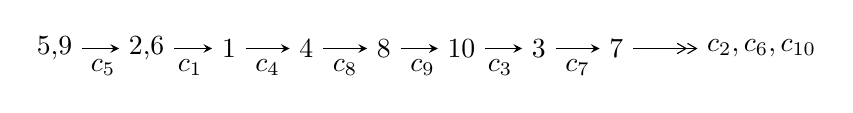
\begin{tikzpicture}[x=28pt, y=7pt]
	% node
	\node (A0) at (-1/8, 0) {5,9};
	\node (A1) at (17/16, 0) {2,6};
	\node (A2) at (17/8, 0) {1};
	\node (A3) at (25/8, 0) {4};
	\node (A4) at (33/8, 0) {8};
	\node (A5) at (41/8, 0) {10};
	\node (A6) at (49/8, 0) {3};
	\node (A7) at (57/8, 0) {7};
	\node (C1) at (1/2, -1) {$c_{5}$};
	\node (C2) at (13/8, -1) {$c_{1}$};
	\node (C3) at (21/8, -1) {$c_{4}$};
	\node (C4) at (29/8, -1) {$c_{8}$};
	\node (C5) at (37/8, -1) {$c_{9}$};
	\node (C6) at (45/8, -1) {$c_{3}$};
	\node (C7) at (53/8, -1) {$c_{7}$};
	\node (A8) at (9, 0) {$c_{2},c_{6},c_{10}$};

	% edge
	\draw[->,>=stealth]	
	(A0) edge (A1) (A1) edge (A2) (A2) edge (A3) (A3) edge (A4) (A4) edge (A5) (A5) edge (A6) (A6) edge (A7) ;
	\draw[->>,>={angle 60}]	
	(A7) edge (A8);
\end{tikzpicture} \\ 

\end{tabular} \\

\footnotetext{
The image of knot diagram is generated by the software ``\textbf{Draw programme}" developed by Andrew Bartholomew(\url{http://www.layer8.co.uk/maths/draw/index.htm\#Running-draw}), where we modified some parts for our purpose(\url{https://github.com/CATsTAILs/LinksPainter}).
}\phantom \\ \newline 
\centering \textbf{Ideals for irreducible components\footnotemark of $X_{\text{par}}$} 
 
\begin{align*}
I^u_{1}&=\langle 
-4.78927\times10^{31} u^{49}+8.64865\times10^{31} u^{48}+\cdots+2.44356\times10^{32} b+3.07584\times10^{32},\\
\phantom{I^u_{1}}&\phantom{= \langle  }-1.85309\times10^{32} u^{49}+2.34614\times10^{31} u^{48}+\cdots+2.44356\times10^{32} a-4.39857\times10^{31},\;u^{50}- u^{49}+\cdots-5 u+1\rangle \\
\\
\end{align*}
\raggedright * 1 irreducible components of $\dim_{\mathbb{C}}=0$, with total 50 representations.\\
\footnotetext{All coefficients of polynomials are rational numbers. But the coefficients are sometimes approximated in decimal forms when there is not enough margin.}
\newpage
\renewcommand{\arraystretch}{1}
\centering \section*{I. $I^u_{1}= \langle -4.79\times10^{31} u^{49}+8.65\times10^{31} u^{48}+\cdots+2.44\times10^{32} b+3.08\times10^{32},\;-1.85\times10^{32} u^{49}+2.35\times10^{31} u^{48}+\cdots+2.44\times10^{32} a-4.40\times10^{31},\;u^{50}- u^{49}+\cdots-5 u+1 \rangle$}
\flushleft \textbf{(i) Arc colorings}\\
\begin{tabular}{m{7pt} m{180pt} m{7pt} m{180pt} }
\flushright $a_{5}=$&$\begin{pmatrix}1\\0\end{pmatrix}$ \\
\flushright $a_{9}=$&$\begin{pmatrix}0\\u\end{pmatrix}$ \\
\flushright $a_{2}=$&$\begin{pmatrix}0.758359 u^{49}-0.0960131 u^{48}+\cdots+4.45061 u+0.180007\\0.195996 u^{49}-0.353937 u^{48}+\cdots+6.62447 u-1.25875\end{pmatrix}$ \\
\flushright $a_{6}=$&$\begin{pmatrix}1\\u^2\end{pmatrix}$ \\
\flushright $a_{1}=$&$\begin{pmatrix}0.562363 u^{49}+0.257923 u^{48}+\cdots-2.17386 u+1.43876\\0.195996 u^{49}-0.353937 u^{48}+\cdots+6.62447 u-1.25875\end{pmatrix}$ \\
\flushright $a_{4}=$&$\begin{pmatrix}0.884162 u^{49}+0.510722 u^{48}+\cdots+10.7623 u-1.94330\\0.177826 u^{49}-0.322317 u^{48}+\cdots+6.18097 u-2.09684\end{pmatrix}$ \\
\flushright $a_{8}=$&$\begin{pmatrix}u\\u^3+u\end{pmatrix}$ \\
\flushright $a_{10}=$&$\begin{pmatrix}u^3\\u^5+u^3+u\end{pmatrix}$ \\
\flushright $a_{3}=$&$\begin{pmatrix}1.04226 u^{49}+0.469203 u^{48}+\cdots+10.2187 u-1.83350\\0.203367 u^{49}-0.392648 u^{48}+\cdots+6.44615 u-2.34009\end{pmatrix}$ \\
\flushright $a_{7}=$&$\begin{pmatrix}-0.870023 u^{49}+1.11164 u^{48}+\cdots-2.30734 u+2.02319\\0.169826 u^{49}-0.715422 u^{48}+\cdots+2.88924 u+0.199819\end{pmatrix}$\\&\end{tabular}
\flushleft \textbf{(ii) Obstruction class $= -1$}\\~\\
\flushleft \textbf{(iii) Cusp Shapes $= 2.37628 u^{49}-0.986125 u^{48}+\cdots-35.4700 u+13.0744$}\\~\\
\newpage\renewcommand{\arraystretch}{1}
\flushleft \textbf{(iv) u-Polynomials at the component}\newline \\
\begin{tabular}{m{50pt}|m{274pt}}
Crossings & \hspace{64pt}u-Polynomials at each crossing \\
\hline $$\begin{aligned}c_{1},c_{4}\end{aligned}$$&$\begin{aligned}
&u^{50}+u^{49}+\cdots+5 u+1
\end{aligned}$\\
\hline $$\begin{aligned}c_{2}\end{aligned}$$&$\begin{aligned}
&u^{50}+21 u^{49}+\cdots+5 u+1
\end{aligned}$\\
\hline $$\begin{aligned}c_{3}\end{aligned}$$&$\begin{aligned}
&u^{50}+5 u^{49}+\cdots+u+1
\end{aligned}$\\
\hline $$\begin{aligned}c_{5},c_{8}\end{aligned}$$&$\begin{aligned}
&u^{50}- u^{49}+\cdots-5 u+1
\end{aligned}$\\
\hline $$\begin{aligned}c_{6}\end{aligned}$$&$\begin{aligned}
&u^{50}+u^{49}+\cdots-17 u+1
\end{aligned}$\\
\hline $$\begin{aligned}c_{7}\end{aligned}$$&$\begin{aligned}
&u^{50}- u^{49}+\cdots+17 u+1
\end{aligned}$\\
\hline $$\begin{aligned}c_{9}\end{aligned}$$&$\begin{aligned}
&u^{50}-21 u^{49}+\cdots-5 u+1
\end{aligned}$\\
\hline $$\begin{aligned}c_{10}\end{aligned}$$&$\begin{aligned}
&u^{50}-5 u^{49}+\cdots- u+1
\end{aligned}$\\
\hline
\end{tabular}\\~\\
\newpage\renewcommand{\arraystretch}{1}
\flushleft \textbf{(v) Riley Polynomials at the component}\newline \\
\begin{tabular}{m{50pt}|m{274pt}}
Crossings & \hspace{64pt}Riley Polynomials at each crossing \\
\hline $$\begin{aligned}c_{1},c_{4},c_{5}\\c_{8}\end{aligned}$$&$\begin{aligned}
&y^{50}+21 y^{49}+\cdots+5 y+1
\end{aligned}$\\
\hline $$\begin{aligned}c_{2},c_{9}\end{aligned}$$&$\begin{aligned}
&y^{50}+17 y^{49}+\cdots-71 y+1
\end{aligned}$\\
\hline $$\begin{aligned}c_{3},c_{10}\end{aligned}$$&$\begin{aligned}
&y^{50}+5 y^{49}+\cdots+5 y+1
\end{aligned}$\\
\hline $$\begin{aligned}c_{6},c_{7}\end{aligned}$$&$\begin{aligned}
&y^{50}+49 y^{49}+\cdots-11 y+1
\end{aligned}$\\
\hline
\end{tabular}\\~\\
\newpage\flushleft \textbf{(vi) Complex Volumes and Cusp Shapes}
$$\begin{array}{c|c|c}  
\text{Solutions to }I^u_{1}& \I (\text{vol} + \sqrt{-1}CS) & \text{Cusp shape}\\
 \hline 
\begin{aligned}
u &= -0.436223 + 0.912127 I \\
a &= -0.05994 + 2.46842 I \\
b &= \phantom{-}0.513623 - 0.775619 I\end{aligned}
 & \phantom{-}0.465700 + 0.257544 I & -10.73692 + 5.77650 I \\ \hline\begin{aligned}
u &= -0.436223 - 0.912127 I \\
a &= -0.05994 - 2.46842 I \\
b &= \phantom{-}0.513623 + 0.775619 I\end{aligned}
 & \phantom{-}0.465700 - 0.257544 I & -10.73692 - 5.77650 I \\ \hline\begin{aligned}
u &= -0.948189 + 0.263019 I \\
a &= \phantom{-}0.47046 + 1.33916 I \\
b &= -0.390240 + 0.977451 I\end{aligned}
 & -3.46714 - 1.26448 I & -10.24310 + 1.49533 I \\ \hline\begin{aligned}
u &= -0.948189 - 0.263019 I \\
a &= \phantom{-}0.47046 - 1.33916 I \\
b &= -0.390240 - 0.977451 I\end{aligned}
 & -3.46714 + 1.26448 I & -10.24310 - 1.49533 I \\ \hline\begin{aligned}
u &= \phantom{-}0.751604 + 0.620367 I \\
a &= \phantom{-}0.76094 + 2.10184 I \\
b &= -0.101263 + 1.224450 I\end{aligned}
 & -5.61738 + 1.76997 I & -6.58185 - 1.55968 I \\ \hline\begin{aligned}
u &= \phantom{-}0.751604 - 0.620367 I \\
a &= \phantom{-}0.76094 - 2.10184 I \\
b &= -0.101263 - 1.224450 I\end{aligned}
 & -5.61738 - 1.76997 I & -6.58185 + 1.55968 I \\ \hline\begin{aligned}
u &= \phantom{-}0.926795 + 0.461408 I \\
a &= \phantom{-}0.06013 - 1.60838 I \\
b &= -0.629982 - 1.117780 I\end{aligned}
 & -2.06994 + 9.79621 I & -2.50765 - 6.28548 I \\ \hline\begin{aligned}
u &= \phantom{-}0.926795 - 0.461408 I \\
a &= \phantom{-}0.06013 + 1.60838 I \\
b &= -0.629982 + 1.117780 I\end{aligned}
 & -2.06994 - 9.79621 I & -2.50765 + 6.28548 I \\ \hline\begin{aligned}
u &= \phantom{-}0.315698 + 0.896805 I \\
a &= \phantom{-}0.094858 - 0.349071 I \\
b &= \phantom{-}0.802649 + 0.956850 I\end{aligned}
 & \phantom{-}2.17019 + 1.69704 I & \phantom{-}6.69422 - 3.84304 I \\ \hline\begin{aligned}
u &= \phantom{-}0.315698 - 0.896805 I \\
a &= \phantom{-}0.094858 + 0.349071 I \\
b &= \phantom{-}0.802649 - 0.956850 I\end{aligned}
 & \phantom{-}2.17019 - 1.69704 I & \phantom{-}6.69422 + 3.84304 I\\
 \hline 
 \end{array}$$\newpage$$\begin{array}{c|c|c}  
\text{Solutions to }I^u_{1}& \I (\text{vol} + \sqrt{-1}CS) & \text{Cusp shape}\\
 \hline 
\begin{aligned}
u &= \phantom{-}0.390240 + 0.977451 I \\
a &= \phantom{-}0.218149 - 0.845172 I \\
b &= \phantom{-}0.948189 + 0.263019 I\end{aligned}
 & \phantom{-}3.46714 - 1.26448 I & \phantom{-}10.24310 + 1.49533 I \\ \hline\begin{aligned}
u &= \phantom{-}0.390240 - 0.977451 I \\
a &= \phantom{-}0.218149 + 0.845172 I \\
b &= \phantom{-}0.948189 - 0.263019 I\end{aligned}
 & \phantom{-}3.46714 + 1.26448 I & \phantom{-}10.24310 - 1.49533 I \\ \hline\begin{aligned}
u &= -0.520399 + 0.919399 I \\
a &= -3.68586 + 2.69325 I \\
b &= \phantom{-}0.520399 + 0.919399 I\end{aligned}
 & \phantom{-0.000000 -}4.46279 I & \phantom{-0.000000 -}0. + 17.3614 I \\ \hline\begin{aligned}
u &= -0.520399 - 0.919399 I \\
a &= -3.68586 - 2.69325 I \\
b &= \phantom{-}0.520399 - 0.919399 I\end{aligned}
 & \phantom{-0.000000 } -4.46279 I & \phantom{-0.000000 } 0. - 17.3614 I \\ \hline\begin{aligned}
u &= \phantom{-}0.836943 + 0.423224 I \\
a &= -0.232872 + 0.578642 I \\
b &= -0.836943 + 0.423224 I\end{aligned}
 & \phantom{-0.000000 -}4.34036 I & \phantom{-0.000000 } 0. - 2.49570 I \\ \hline\begin{aligned}
u &= \phantom{-}0.836943 - 0.423224 I \\
a &= -0.232872 - 0.578642 I \\
b &= -0.836943 - 0.423224 I\end{aligned}
 & \phantom{-0.000000 } -4.34036 I & \phantom{-0.000000 -}0. + 2.49570 I \\ \hline\begin{aligned}
u &= -0.513623 + 0.775619 I \\
a &= \phantom{-}0.12952 - 3.57817 I \\
b &= \phantom{-}0.436223 - 0.912127 I\end{aligned}
 & -0.465700 - 0.257544 I & \phantom{-}10.73692 - 5.77650 I \\ \hline\begin{aligned}
u &= -0.513623 - 0.775619 I \\
a &= \phantom{-}0.12952 + 3.57817 I \\
b &= \phantom{-}0.436223 + 0.912127 I\end{aligned}
 & -0.465700 + 0.257544 I & \phantom{-}10.73692 + 5.77650 I \\ \hline\begin{aligned}
u &= -0.428462 + 0.986061 I \\
a &= \phantom{-}0.384178 - 0.243345 I \\
b &= \phantom{-}0.151838 + 0.411336 I\end{aligned}
 & \phantom{-}0.42985 + 2.78493 I & -1.80718 - 4.91633 I \\ \hline\begin{aligned}
u &= -0.428462 - 0.986061 I \\
a &= \phantom{-}0.384178 + 0.243345 I \\
b &= \phantom{-}0.151838 - 0.411336 I\end{aligned}
 & \phantom{-}0.42985 - 2.78493 I & -1.80718 + 4.91633 I\\
 \hline 
 \end{array}$$\newpage$$\begin{array}{c|c|c}  
\text{Solutions to }I^u_{1}& \I (\text{vol} + \sqrt{-1}CS) & \text{Cusp shape}\\
 \hline 
\begin{aligned}
u &= \phantom{-}0.454209 + 0.992717 I \\
a &= -0.797222 - 0.884708 I \\
b &= \phantom{-}0.963579 - 0.664758 I\end{aligned}
 & \phantom{-}3.06399 - 4.68595 I & \phantom{-}8.49449 + 8.00357 I \\ \hline\begin{aligned}
u &= \phantom{-}0.454209 - 0.992717 I \\
a &= -0.797222 + 0.884708 I \\
b &= \phantom{-}0.963579 + 0.664758 I\end{aligned}
 & \phantom{-}3.06399 + 4.68595 I & \phantom{-}8.49449 - 8.00357 I \\ \hline\begin{aligned}
u &= \phantom{-}0.534615 + 0.993631 I \\
a &= -1.49902 - 1.80771 I \\
b &= \phantom{-}0.669156 - 1.208830 I\end{aligned}
 & \phantom{-}0.67245 - 7.17988 I & \phantom{-}2.47305 + 11.09561 I \\ \hline\begin{aligned}
u &= \phantom{-}0.534615 - 0.993631 I \\
a &= -1.49902 + 1.80771 I \\
b &= \phantom{-}0.669156 + 1.208830 I\end{aligned}
 & \phantom{-}0.67245 + 7.17988 I & \phantom{-}2.47305 - 11.09561 I \\ \hline\begin{aligned}
u &= -0.634283 + 0.564662 I \\
a &= \phantom{-}0.415195 + 0.219909 I \\
b &= -0.371567 + 0.059094 I\end{aligned}
 & -1.12648 + 1.44226 I & -2.47190 - 3.48786 I \\ \hline\begin{aligned}
u &= -0.634283 - 0.564662 I \\
a &= \phantom{-}0.415195 - 0.219909 I \\
b &= -0.371567 - 0.059094 I\end{aligned}
 & -1.12648 - 1.44226 I & -2.47190 + 3.48786 I \\ \hline\begin{aligned}
u &= -0.963579 + 0.664758 I \\
a &= \phantom{-}0.48756 - 1.58137 I \\
b &= -0.454209 - 0.992717 I\end{aligned}
 & -3.06399 + 4.68595 I & -8.49449 - 8.00357 I \\ \hline\begin{aligned}
u &= -0.963579 - 0.664758 I \\
a &= \phantom{-}0.48756 + 1.58137 I \\
b &= -0.454209 + 0.992717 I\end{aligned}
 & -3.06399 - 4.68595 I & -8.49449 + 8.00357 I \\ \hline\begin{aligned}
u &= \phantom{-}0.646221 + 1.007930 I \\
a &= -0.91233 - 1.58912 I \\
b &= -0.016221 - 1.300020 I\end{aligned}
 & -4.44668 - 7.08217 I & -4.03427 + 7.44469 I \\ \hline\begin{aligned}
u &= \phantom{-}0.646221 - 1.007930 I \\
a &= -0.91233 + 1.58912 I \\
b &= -0.016221 + 1.300020 I\end{aligned}
 & -4.44668 + 7.08217 I & -4.03427 - 7.44469 I\\
 \hline 
 \end{array}$$\newpage$$\begin{array}{c|c|c}  
\text{Solutions to }I^u_{1}& \I (\text{vol} + \sqrt{-1}CS) & \text{Cusp shape}\\
 \hline 
\begin{aligned}
u &= \phantom{-}0.101263 + 1.224450 I \\
a &= \phantom{-}0.961820 + 0.164264 I \\
b &= -0.751604 + 0.620367 I\end{aligned}
 & \phantom{-}5.61738 + 1.76997 I & \phantom{-}6.58185 - 1.55968 I \\ \hline\begin{aligned}
u &= \phantom{-}0.101263 - 1.224450 I \\
a &= \phantom{-}0.961820 - 0.164264 I \\
b &= -0.751604 - 0.620367 I\end{aligned}
 & \phantom{-}5.61738 - 1.76997 I & \phantom{-}6.58185 + 1.55968 I \\ \hline\begin{aligned}
u &= -0.802649 + 0.956850 I \\
a &= -0.154615 + 1.120140 I \\
b &= -0.315698 + 0.896805 I\end{aligned}
 & -2.17019 + 1.69704 I & -6.69422 + 0. I\phantom{ +0.000000I} \\ \hline\begin{aligned}
u &= -0.802649 - 0.956850 I \\
a &= -0.154615 - 1.120140 I \\
b &= -0.315698 - 0.896805 I\end{aligned}
 & -2.17019 - 1.69704 I & -6.69422 + 0. I\phantom{ +0.000000I} \\ \hline\begin{aligned}
u &= -0.518931 + 1.139540 I \\
a &= \phantom{-}0.281111 - 0.250166 I \\
b &= -0.441150 + 0.556001 I\end{aligned}
 & \phantom{-}0.60255 + 2.94954 I & \phantom{-0.000000 } 0. - 5.37680 I \\ \hline\begin{aligned}
u &= -0.518931 - 1.139540 I \\
a &= \phantom{-}0.281111 + 0.250166 I \\
b &= -0.441150 - 0.556001 I\end{aligned}
 & \phantom{-}0.60255 - 2.94954 I & \phantom{-0.000000 -}0. + 5.37680 I \\ \hline\begin{aligned}
u &= \phantom{-}0.629982 + 1.117780 I \\
a &= -0.238857 + 0.640097 I \\
b &= -0.926795 - 0.461408 I\end{aligned}
 & \phantom{-}2.06994 - 9.79621 I & \phantom{-0.000000 } 0 \\ \hline\begin{aligned}
u &= \phantom{-}0.629982 - 1.117780 I \\
a &= -0.238857 - 0.640097 I \\
b &= -0.926795 + 0.461408 I\end{aligned}
 & \phantom{-}2.06994 + 9.79621 I & \phantom{-0.000000 } 0 \\ \hline\begin{aligned}
u &= \phantom{-}0.441150 + 0.556001 I \\
a &= \phantom{-}0.89388 + 1.68739 I \\
b &= \phantom{-}0.518931 + 1.139540 I\end{aligned}
 & -0.60255 + 2.94954 I & -1.13612 - 5.37680 I \\ \hline\begin{aligned}
u &= \phantom{-}0.441150 - 0.556001 I \\
a &= \phantom{-}0.89388 - 1.68739 I \\
b &= \phantom{-}0.518931 - 1.139540 I\end{aligned}
 & -0.60255 - 2.94954 I & -1.13612 + 5.37680 I\\
 \hline 
 \end{array}$$\newpage$$\begin{array}{c|c|c}  
\text{Solutions to }I^u_{1}& \I (\text{vol} + \sqrt{-1}CS) & \text{Cusp shape}\\
 \hline 
\begin{aligned}
u &= \phantom{-}0.016221 + 1.300020 I \\
a &= \phantom{-}0.841104 - 0.210805 I \\
b &= -0.646221 - 1.007930 I\end{aligned}
 & \phantom{-}4.44668 + 7.08217 I & \phantom{-0.000000 } 0. - 7.44469 I \\ \hline\begin{aligned}
u &= \phantom{-}0.016221 - 1.300020 I \\
a &= \phantom{-}0.841104 + 0.210805 I \\
b &= -0.646221 + 1.007930 I\end{aligned}
 & \phantom{-}4.44668 - 7.08217 I & \phantom{-0.000000 -}0. + 7.44469 I \\ \hline\begin{aligned}
u &= \phantom{-}0.670825 + 1.138630 I \\
a &= \phantom{-}1.49989 + 1.65059 I \\
b &= -0.670825 + 1.138630 I\end{aligned}
 & \phantom{-0.000000 } -15.6466 I & \phantom{-0.000000 } 0 \\ \hline\begin{aligned}
u &= \phantom{-}0.670825 - 1.138630 I \\
a &= \phantom{-}1.49989 - 1.65059 I \\
b &= -0.670825 - 1.138630 I\end{aligned}
 & \phantom{-0.000000 -}15.6466 I & \phantom{-0.000000 } 0 \\ \hline\begin{aligned}
u &= -0.669156 + 1.208830 I \\
a &= \phantom{-}1.36920 - 1.22455 I \\
b &= -0.534615 - 0.993631 I\end{aligned}
 & -0.67245 + 7.17988 I & \phantom{-0.000000 } 0 \\ \hline\begin{aligned}
u &= -0.669156 - 1.208830 I \\
a &= \phantom{-}1.36920 + 1.22455 I \\
b &= -0.534615 + 0.993631 I\end{aligned}
 & -0.67245 - 7.17988 I & \phantom{-0.000000 } 0 \\ \hline\begin{aligned}
u &= -0.151838 + 0.411336 I \\
a &= \phantom{-}1.52157 + 0.76573 I \\
b &= \phantom{-}0.428462 + 0.986061 I\end{aligned}
 & -0.42985 + 2.78493 I & \phantom{-}1.80718 - 4.91633 I \\ \hline\begin{aligned}
u &= -0.151838 - 0.411336 I \\
a &= \phantom{-}1.52157 - 0.76573 I \\
b &= \phantom{-}0.428462 - 0.986061 I\end{aligned}
 & -0.42985 - 2.78493 I & \phantom{-}1.80718 + 4.91633 I \\ \hline\begin{aligned}
u &= \phantom{-}0.371567 + 0.059094 I \\
a &= \phantom{-}1.69115 + 0.65214 I \\
b &= \phantom{-}0.634283 + 0.564662 I\end{aligned}
 & \phantom{-}1.12648 + 1.44226 I & \phantom{-}2.47190 - 3.48786 I \\ \hline\begin{aligned}
u &= \phantom{-}0.371567 - 0.059094 I \\
a &= \phantom{-}1.69115 - 0.65214 I \\
b &= \phantom{-}0.634283 - 0.564662 I\end{aligned}
 & \phantom{-}1.12648 - 1.44226 I & \phantom{-}2.47190 + 3.48786 I\\
 \hline 
 \end{array}$$\newpage
\newpage\renewcommand{\arraystretch}{1}
\centering \section*{ II. u-Polynomials}
\begin{tabular}{m{50pt}|m{274pt}}
Crossings & \hspace{64pt}u-Polynomials at each crossing \\
\hline $$\begin{aligned}c_{1},c_{4}\end{aligned}$$&$\begin{aligned}
&u^{50}+u^{49}+\cdots+5 u+1
\end{aligned}$\\
\hline $$\begin{aligned}c_{2}\end{aligned}$$&$\begin{aligned}
&u^{50}+21 u^{49}+\cdots+5 u+1
\end{aligned}$\\
\hline $$\begin{aligned}c_{3}\end{aligned}$$&$\begin{aligned}
&u^{50}+5 u^{49}+\cdots+u+1
\end{aligned}$\\
\hline $$\begin{aligned}c_{5},c_{8}\end{aligned}$$&$\begin{aligned}
&u^{50}- u^{49}+\cdots-5 u+1
\end{aligned}$\\
\hline $$\begin{aligned}c_{6}\end{aligned}$$&$\begin{aligned}
&u^{50}+u^{49}+\cdots-17 u+1
\end{aligned}$\\
\hline $$\begin{aligned}c_{7}\end{aligned}$$&$\begin{aligned}
&u^{50}- u^{49}+\cdots+17 u+1
\end{aligned}$\\
\hline $$\begin{aligned}c_{9}\end{aligned}$$&$\begin{aligned}
&u^{50}-21 u^{49}+\cdots-5 u+1
\end{aligned}$\\
\hline $$\begin{aligned}c_{10}\end{aligned}$$&$\begin{aligned}
&u^{50}-5 u^{49}+\cdots- u+1
\end{aligned}$\\
\hline
\end{tabular}\newpage\renewcommand{\arraystretch}{1}
\centering \section*{ III. Riley Polynomials}
\begin{tabular}{m{50pt}|m{274pt}}
Crossings & \hspace{64pt}Riley Polynomials at each crossing \\
\hline $$\begin{aligned}c_{1},c_{4},c_{5}\\c_{8}\end{aligned}$$&$\begin{aligned}
&y^{50}+21 y^{49}+\cdots+5 y+1
\end{aligned}$\\
\hline $$\begin{aligned}c_{2},c_{9}\end{aligned}$$&$\begin{aligned}
&y^{50}+17 y^{49}+\cdots-71 y+1
\end{aligned}$\\
\hline $$\begin{aligned}c_{3},c_{10}\end{aligned}$$&$\begin{aligned}
&y^{50}+5 y^{49}+\cdots+5 y+1
\end{aligned}$\\
\hline $$\begin{aligned}c_{6},c_{7}\end{aligned}$$&$\begin{aligned}
&y^{50}+49 y^{49}+\cdots-11 y+1
\end{aligned}$\\
\hline
\end{tabular}
\vskip 2pc
\end{document}